\chapter{Le gestionnaire de paquets }
\minitoc
\clearpage

\label{sec:kraken-pkg}
\section{Introduction}
Un gestionnaire de paquets est un outil  permettant d’automatiser les processus d’installation, de mise à jour et de suppression de paquets sur un système Linux. 

Malheureusement, le mécanisme de gestion des paquets n’est pas un aspect purement théorique. En pratique, chaque grande distribution conçoit son propre gestionnaire de paquets, selon une philosophie qui lui est propre.\\
À ce stade, il est donc important de comprendre que nous devons inventer un nouveau gestionnaire de paquets conçu et développé entièrement à partir de zéro, sans s’appuyer sur
un autre gestionnaire existant

L’objectif du gestionnaire de paquets \textsc{Kraken} est de fournir une solution à la fois simple et efficace pour l’installation, la mise à jour, la configuration et la suppression des logiciels. Il prend en charge les dépendances, la gestion des versions, ainsi que toutes les tâches complexes afin de faciliter la gestion des programmes.



%\subsection{Fonctionnalités du gestionnaire de paquets sous Linux}
%\label{subsec:kraken-fonctions}

%\begin{itemize}
 % \item \textbf{Installation}  
  %  Permet d’installer des paquets depuis des dépôts distants . Gère automatiquement les dépendances
  %\item \textbf{Résolution de dépendances}  
  %  Analyse les besoins de chaque paquet et récupère automatiquement les paquets requis.
  %\item \textbf{Mise à jour (upgrade)}  
  %  Met à jour les paquets installés vers leurs dernières versions, assurant ainsi la sécurité et la fraîcheur du système.
  %\item \textbf{Suppression}  
  %  Désinstalle les paquets et leurs dépendances obsolètes, sans laisser de fichiers orphelins.
  %\item \textbf{Interrogation (query)}  
  %  Fournit des commandes pour lister les paquets installés, les mises à jour disponibles et les détails de %chaque paquet.
%\end{itemize}



\section{ Architecture du  la gestionnaire de paquets }


 


\begin{figure}[H]
  \centering
  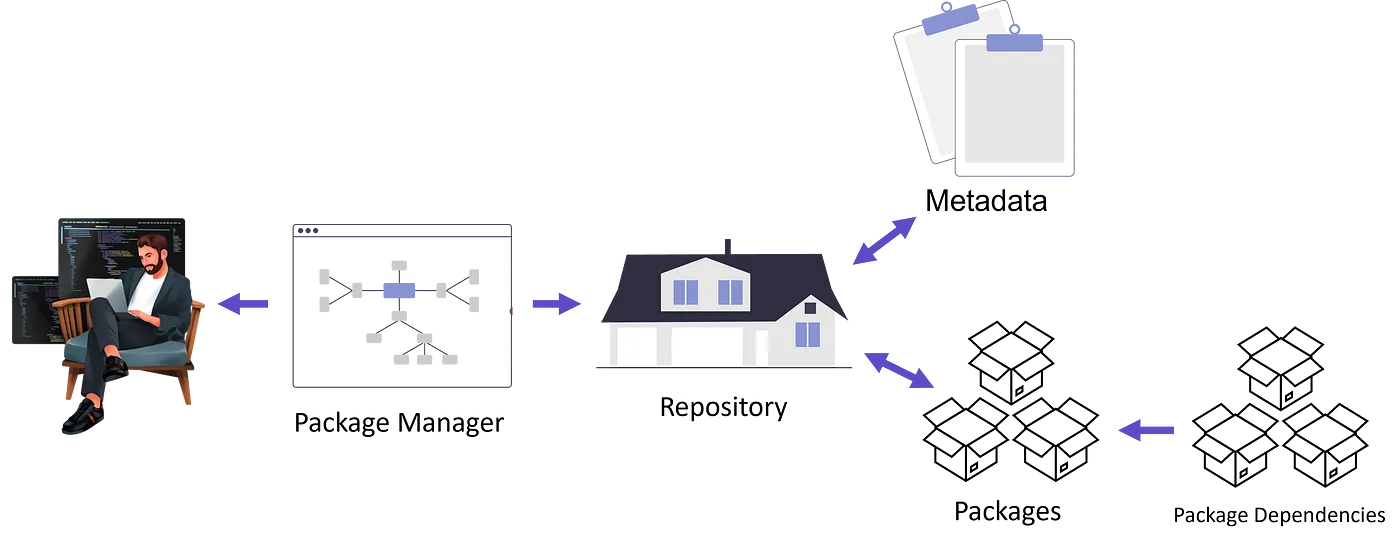
\includegraphics[width=0.85\textwidth]{images_pfe/packagemanager.png}
  \caption{ Architecture gestionnaire de paquets }
  \label{fig:packagemanager}
\end{figure}


 Cette figure illustre la manière dont nous avons conçu notre gestionnaire de paquets. 
 Le premier composant de Kraken est le \textbf{dépôt} (Repository) , où sont stockées les métadonnées des paquets. Chaque paquet est décrit par un fichier \textbf{pkgbuild.kraken}(metadata), qui définit la procédure d'installation du paquet sur notre  à l'aide du gestionnaire de paquets Kraken. \\
 Le deuxième composant correspond aux \textbf{outils du gestionnaire de paquets}, qui permettent de récupérer, interroger et installer les paquets depuis le dépôt vers le système. 

Avant de commencer à développer le gestionnaire de paquets \textsc{Kraken}, il est essentiel de comprendre un problème majeur connu sous le nom de \textbf{« dependency hell »} (l’enfer des dépendances).

\section{Qu’est‑ce qu’une dépendance de paquet ?}
\label{subsec:dependency}

Une dépendance de paquet est l’ensemble des autres paquets, bibliothèques ou outils requis pour qu’un paquet puisse s’installer et fonctionner correctement. Pour installer un paquet, il faut résoudre automatiquement toutes ses dépendances dans le bon ordre. 

On peut visualiser ce processus comme un graphe orienté : chaque nœud représente un paquet, et chaque arc pointe vers un paquet dont il dépend.  

\begin{figure}[H]
  \centering
  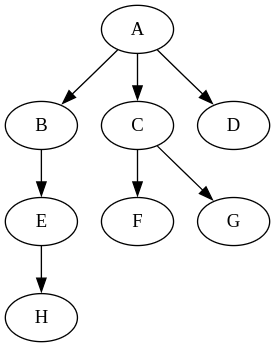
\includegraphics[width=0.5\textwidth , height=10cm]{images_pfe/genralgraphexemple.png}
  \caption{Exemple de graphe de dépendances}
  \label{fig:exempledepndencygraph}
\end{figure}


Pour installer le paquet \texttt{A} :
\begin{enumerate}
  \item Il faut d’abord installer \texttt{B}, \texttt{C} et \texttt{D}.
  \item Pour \texttt{B}, on doit installer \texttt{E}, lui‑même dépendant de \texttt{H}.
  \item Une fois \texttt{B}  installés, on revient au sous‑graphe de \texttt{C} et on installe \texttt{F} et \texttt{G}.
\end{enumerate}

Cette résolution suit en général un algorithme de \textbf{parcours en profondeur} (DFS) du graphe de dépendances.  

Cependant, dans la pratique, le graphe peut être très vaste (des dizainess de paquets) et contenir  des cycle. Il faut alors mettre en place des stratégies d’optimisation (caching, détection de cycles, etc.). Tous ces enjeux sont regroupés sous le terme \textbf{« enfer des dépendances »} (Dependency Hell).


\subsection{Premier problème : dépendances circulaires}
\label{subsec:circular-dependencies}

Une dépendance circulaire survient lorsqu’un paquet A dépend d’un paquet B, qui lui-même dépend de A. Cette situation bloque la résolution automatique des dépendances, car ni A ni B ne peut être installé en premier sans l’autre.

\begin{figure}[H]
  \centering
  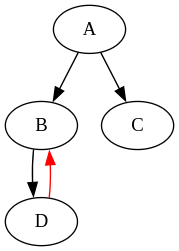
\includegraphics[width=0.3\textwidth, height=8cm]{images_pfe/CERCULARDEP.png}
  \caption{Exemple simple de dépendance circulaire}
  \label{fig:circular-dep}
\end{figure}



Sur la figure~\textcolor{blue}{\ref{fig:circular-dep}}, pour installer \texttt{B}, il faut d’abord installer \texttt{D}, qui dépend de \texttt{B}, bouclant ainsi le processus.

\paragraph{Cas d’usage réel : outils multimédia}
Considérons deux paquets :
\begin{itemize}
  \item \textbf{DocumentConverter} : convertit des documents (PDF → Word, etc.) et nécessite \texttt{FileViewer} pour prévisualiser les fichiers convertis.
  \item \textbf{FileViewer} : affiche des documents (PDF, Word, ODT, etc.) et nécessite \texttt{DocumentConverter} pour convertir les \textbf{formats non pris en charge}.
\end{itemize}

\begin{figure}[H]
  \centering
  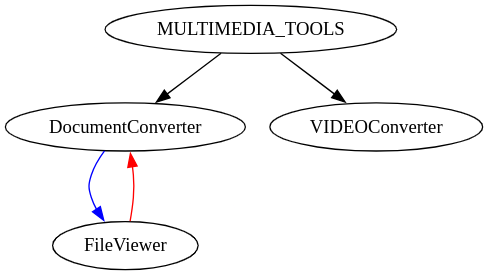
\includegraphics[width=0.5\textwidth]{images_pfe/depcycleexemple.png}
  \caption{Boucle de dépendance entre \texttt{DocumentConverter} et \texttt{FileViewer}}
  \label{fig:depcycle-multimedia}
\end{figure}



\subsubsection*{Stratégie de résolution}
Pour casser la boucle de dépendances, on procède en plusieurs étapes :
\begin{enumerate}
  \item \textbf{Installation initiale de FileViewer (minimal)}  
    Compiler et installer \texttt{FileViewer} \textbf{sans} le support de conversion.
  \item \textbf{Installation de DocumentConverter}  
    Compiler et installer \texttt{DocumentConverter}, qui s’appuie sur le FileViewer minimal.
  \item \textbf{Recompilation de FileViewer}  
    Recompiler \texttt{FileViewer} en activant le support de \texttt{DocumentConverter}.
  \item \textbf{Installation finale de FileViewer complet}  
    Installer la nouvelle version de \texttt{FileViewer} avec toutes les fonctionnalités.
\end{enumerate}

Cette méthode garantit que chaque paquet et ses dépendances sont disponibles au moment opportun, évitant ainsi l’« enfer des dépendances » engendré par les boucles circulaires. 



\subsection{Deuxième problème : conflit de dépendances}
\label{subsec:dependency-conflict}

Un conflit de dépendances survient lorsque deux paquets, ou plus, requièrent la même bibliothèque ou le même composant, mais chacun spécifie une version différente. Par exemple, sur la figure~\textcolor{blue}{\ref{fig:dependency-conflict}} :

\begin{figure}[H]
  \centering
  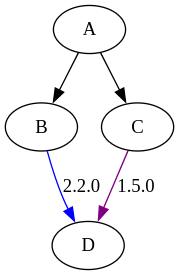
\includegraphics[width=0.3\textwidth, height=5cm]{images_pfe/dpendencyconfligt.png}
  \caption{Exemple de conflit de dépendances }
  \label{fig:dependency-conflict}
\end{figure}

Ici, \texttt{B} dépend de \texttt{D} en version 2.2.0, alors que \texttt{C} exige la version 1.5.0. Le gestionnaire doit alors choisir :

\begin{itemize}
  \item Installer la version la plus récente (2.2.0), au risque de casser \texttt{C}.
  \item Installer la version la plus ancienne (1.5.0), au risque de manquer des correctifs ou fonctionnalités pour \texttt{B}.
  \item Installer simultanément les deux versions, .  au risque de conflit dans le systeme
\end{itemize}

\subsubsection*{Stratégies de résolution}

Malheureusement, ce problème est, pour moi, un problème non résolu en informatique. J'ai effectué de nombreuses recherches pour tenter de trouver une solution, mais chaque gestionnaire de paquets essaie seulement de le contourner sans réellement parvenir à une solution pratique.\\ En général, ils se contentent d'afficher un message à l'utilisateur pour l'informer qu’un conflit existe entre deux ou plusieurs paquets. C’est également l’approche que nous avons choisie. Par exemple, le gestionnaire de paquets \texttt{pacman} de archlinux ou encore \texttt{xbps} de Void Linux adoptent cette stratégie.




\section{Pourquoi avons-nous besoin d’un mécanisme de suivi des métadonnées des paquets ?}
\label{subsec:suivi-fichiers}

Dans un système Linux, l’installation d’un paquet répartit ses fichiers sur de nombreux emplacements :
\begin{itemize}
  \item Binaires : \texttt{/usr/bin}, \texttt{/usr/local/bin}, etc.  
  \item Bibliothèques : \texttt{/lib}, \texttt{/usr/lib}, \texttt{/lib64}, etc.  
  \item En-têtes : \texttt{/usr/include}, etc.  
  \item Fichiers de configuration : \texttt{/etc}.  
  \item Documentation : \texttt{/usr/share/doc}, \texttt{/usr/share/man}, etc.  
  \item Éléments supplémentaires : \texttt{/opt}, \texttt{/var}, etc.  
\end{itemize}

Sans mécanisme de suivi, désinstaller proprement un paquet devient fastidieux : il faudrait rechercher manuellement chacun de ses fichiers dans tout le système, ce qui est impraticable quand on gère des centaines de milliers de fichiers.

\textbf{Notre solution :} développer un mécanisme de « fausse installation ». Ce mécanisme doit générer des fichiers de métadonnées contenant tous les chemins des fichiers et répertoires créés ou modifiés lors de l’installation du paquet. \textbf{Nous détaillerons cette approche dans le section} \textcolor{blue}{\ref{subsecc:fakeinstall}} .
\section{Conclusion}
Le gestionnaire de paquets est l'un des composants les plus complexes et cruciaux d'une distribution Linux. Il nécessite une approche rigoureuse , surtout lorsqu'il s'agit de construire les paquets à partir des sources. \\
En effet, une simple erreur dans ce composant peut compromettre le système entier, le rendant inutilisable.



\clearpage